\section{Introduction}

\label{intro}

To start on this long way we will focus on the principal key words of this Thesis.

\vspace{5 mm}

\noindent These are: 

\begin{itemize}
\item White Rabbit Project
\begin{itemize}
\item Synchronous Ethernet (SyncE) 
\item PTP (Precision Time Protocol) 
\item EtherBone Core
\item Chronos Project
\end{itemize}
\item SPAD Sensors
\item TSN
\item RISC-V.
\item Neuromorphic Sensors
\end{itemize}

\subsection{White Rabbit Project}

The White Rabbit Project \cite{white-rabbit} is a high-precision synchronization system developed by CERN (the European Organization for Nuclear Research).
It’s designed to achieve extremely accurate time synchronization across \textbf{distributed networks}. 
Specifically, it combines Ethernet and Synchronous Ethernet (SyncE) technologies with PTP (Precision Time Protocol), creating what is known as the \say{White Rabbit Protocol}.
The primary goal is to ensure that all connected devices are synchronized within sub-nanosecond accuracy.

\vspace{5 mm}

\noindent According to this ICALPECS 2011 poster (13th International Conference on Accelerator and Large Experimental Physics Control Systems) \cite{white-rabbit:poster}, titled \say{Reliability
in a White Rabbit Network}, White Rabbit (WR) is a time-deterministic, low-latency Ethernet-based network which enables transparent, sub-ns accuracy timing distribution. 
It is being developed to replace the General Machine Timing (GMT) system currently (2011) used at CERN and will become the foundation for the control system of the Facility for Antiproton and Ion Research (FAIR) at GSI.
High reliability is an important issue in WR’s design, since unavailability of the accelerator’s control system will directly translate into expensive downtime of the machine.

\vspace{5 mm}

\noindent Principal characteristics:

\begin{itemize}
\item High Synchronization Precision
    \begin{itemize}
    \item[>] White Rabbit achieves sub-nanosecond precision in synchronizing all nodes within a network, making it essential for particle physics experiments where precise timing is critical.
    \end{itemize}
\item High Time and Frequency Distribution
    \begin{itemize}
    \item[>] White Rabbit enables not only time synchronization but also frequency distribution across devices.
    \item[>] This capability is valuable in scientific experiments, advanced telecommunications, and financial systems where every microsecond matters.
    \end{itemize}
\item Based on Open Standards
    \begin{itemize}
    \item[>] White Rabbit uses open standards, which makes it easy to adopt and adapt to different environments. 
    \item[>] It’s an Open Source hardware and software system, allowing the scientific and tech communities to improve and customize it.
    \end{itemize}
\item Optical Fiber Delay Compensation
    \begin{itemize}
    \item[>] To achieve such high precision, White Rabbit measures and compensates for delays in optical fiber cables, eliminating latency variations that occur over long distances.
    \end{itemize}
\end{itemize}

\vspace{5 mm}

\noindent White Rabbit has been adopted across multiple sectors, including:

\begin{itemize}
\item Scientific Research
    \begin{itemize}
    \item[>] At CERN and other particle physics labs, White Rabbit is crucial for synchronizing detectors, sensors, and other distributed devices in large experimental facilities.
    \end{itemize}
\item Telecommunications
    \begin{itemize}
    \item[>] Telecom providers use White Rabbit to enhance network synchronization accuracy, particularly in \textbf{5G networks} and low-latency services.
    \end{itemize}
\item Industrial Automation
    \begin{itemize}
    \item[>] In production environments, precise synchronization between machines and control systems improves efficiency and reduces errors.
    \end{itemize}
\item Finance
    \begin{itemize}
    \item[>] In finance, where precise timing is critical for high-frequency trading (HFT), White Rabbit enables superior timestamp accuracy.
    \end{itemize}
\end{itemize}

\subsubsection{Synchronous Ethernet (SyncE)}

\subsubsection{PTP (Precision Time Protocol)}

\subsubsection{EtherBone Core}

Etherbone \cite{gl:etherbone-core} is an FPGA-core that connects Ethernet to internal on-chip wishbone buses permitting any core to talk to any other across Ethernet.

\subsubsection{Chronos Project}

Chronos is an advanced timing and synchronization project at CERN, designed to support extremely precise timekeeping requirements in high-energy physics experiments. 

\vspace{5 mm}

\noindent Built on the foundations of the White Rabbit Project, Chronos \cite{gl:chronos} aims to improve upon CERN’s existing timing systems by achieving even more refined synchronization, essential for coordinating complex experiments and data acquisition across CERN’s infrastructure.

\subsection{SPAD Sensors}

SPAD (Single-Photon Avalanche Diode) \cite{9031298} sensors are an advanced type of photodiode sensor, specifically designed to detect extremely low amounts of light, to the single photon level. 
This makes them ideal for applications requiring exceptional sensitivity and the ability to measure extremely \textbf{fast} light events.

\vspace{5 mm}

\noindent Characteristics and Operation of SPADs:

\begin{itemize}
\item High Sensitivity
    \begin{itemize}
    \item[>] SPAD sensors can detect single photons, thanks to their ability to produce an \say{avalanche} of current when a single photon is detected.
    \item[>] This mechanism allows the sensor to significantly amplify the photon signal, providing a clear and strong response.
    \end{itemize}
\item Fast Response Time
    \begin{itemize}
    \item[>] SPADs are capable of recording events in times on the order of picoseconds.
    \item[>] This is useful in applications that require accurate photon arrival time (known as Time-of-Flight or TOF) measurements, such as in LIDAR and Time-Correlated Single Photon Counting (TCSPC), which is used in fluorescence studies.
    \end{itemize}
\item Geiger Mode Operation
    \begin{itemize}
    \item[>] SPADs operate in \say{Geiger} mode, which means that they are polarized at a voltage above the breakdown voltage. 
    \item[>] This causes an electron avalanche when a photon is detected, which allows the detection of the photon to be clearly recorded.
    \item[>] After detection, the sensor \textbf{needs a reset} to be ready for the next event.
    \end{itemize}
\item Dark noise/dark count noise
    \begin{itemize}
    \item[>] Although SPADs are very sensitive, they can suffer from “dark noise”, i.e. false signals caused by thermal electrons in the absence of light. 
    \item[>] This can be significantly controlled with cooling systems or by using signal processing techniques to filter out false events.
    \end{itemize}
\end{itemize}

\vspace{5 mm}

\noindent SPAD Sensor Applications:

\vspace{5 mm}

\noindent SPAD sensors are useful in many areas because of their their photon-level light detection capability and fast response.

\begin{itemize}
\item LIDAR (Light Detection and Ranging)
    \begin{itemize}
    \item[>] SPADs are an ideal choice for high-precision LIDAR systems that measure distances based on the time of flight of reflected photons. 
    \item[>] This is useful in autonomous vehicles, mapping, and environmental monitoring.
    \end{itemize}
\item Biomedicine and Microscopy
    \begin{itemize}
    \item[>] In fluorescence microscopy, SPADs are used for precise photon detection in molecular dynamics studies, where scientists analyze how molecules interact as a function of time.
    \end{itemize}
\item Time-of-Flight (ToF) cameras
    \begin{itemize}
    \item[>] These cameras, which are used in smartphones and augmented reality devices, employ SPAD sensors to capture \textbf{depth information}.
    \item[>] This allows measuring the distance to each point in the image, creating 3-D maps of the environment.
    \end{itemize}
\item Quantum Communications
    \begin{itemize}
    \item[>] SPADs are essential in quantum communications and quantum cryptography, as they can detect single photons that carry quantum information without loss of the signal integrity.
    \end{itemize}
\end{itemize}

\vspace{5 mm}

\noindent Advantages and Disadvantages

\begin{itemize}
\item Advantages:
    \begin{itemize}
    \item[>] Extreme photon sensitivity, appropriate for low light conditions.
    \item[>] Ultra-fast response time, ideal for precise detection and analysis applications.
    \item[>] Quantum information processing capability, important in cryptography and fundamental science.
    \end{itemize}
\item Disadvantages:
    \begin{itemize}
    \item[>] Dark noise, which can limit its accuracy if not properly controlled.
    \item[>] Cost and complexity of manufacture, making them more expensive than other conventional light sensors.
    \item[>] Need for cooling systems in applications where dark noise is critical, which can complicate system design.
    \end{itemize}
\end{itemize}

\subsection{TSN}

\subsection{RISC-V}

\subsection{Neuromorphic Sensors}

\newpage

\section{ASIC}

\begin{figure}[H]
    \centering
    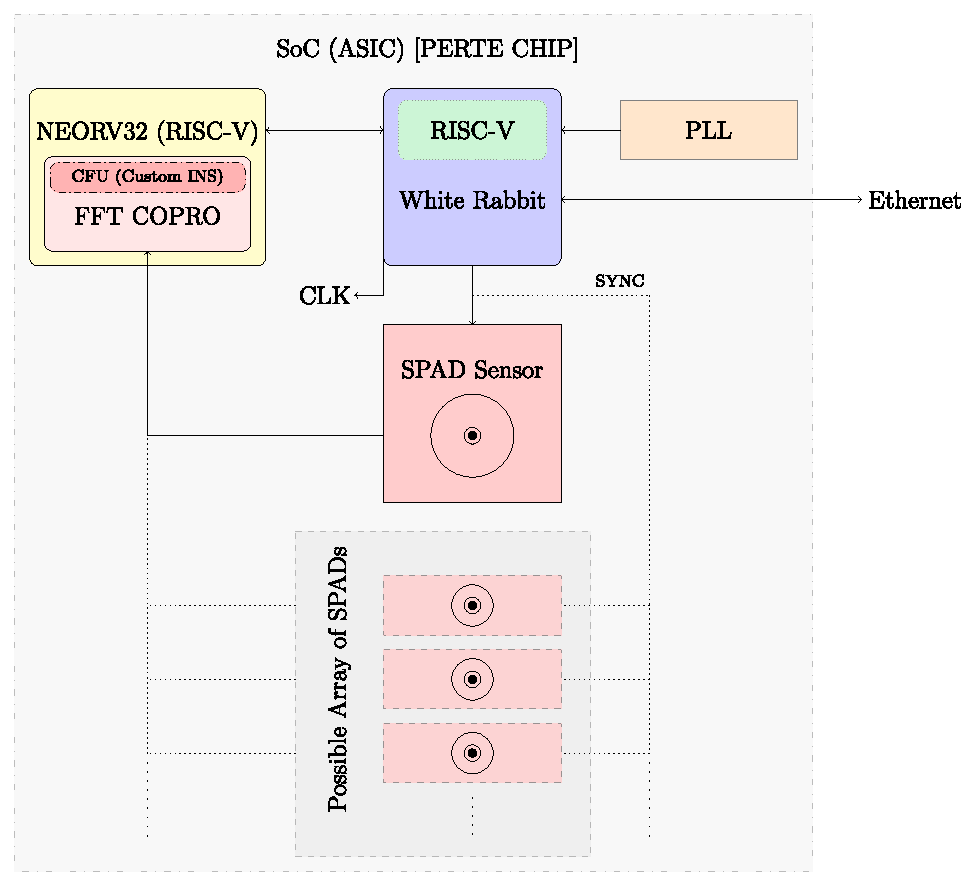
\includegraphics[width=14cm]{figures/ASIC-Scheme.pdf}
    \caption{ASIC a desarrollar.}
    \label{fig:ASIC}
\end{figure}

